We use vue.js (TODO citation) as the UI framework for our tool, combined with PrimeVue (TODO citation) as the UI component library and Tailwind CSS (TODO citation) for CSS utility.
A detailed list of all libraries used can be found in the wiki of our GitHub repository (TODO link).
Table~\ref{tab:libraries} shows an overview of the most important libraries used and their purpose.

% todo insert most important libraries used and their purpose
\begin{table}[!t]
    \caption{Libraries used in the implementation of our tool}
    \label{tab:libraries}
    \centering
    \begin{tabular}{ll}
        \toprule
        \textbf{Library} & \textbf{Purpose}     \\
        \midrule
        vue.js           & UI framework         \\
        PrimeVue         & UI component library \\
        Tailwind CSS     & CSS utility          \\
        \bottomrule
    \end{tabular}
\end{table}

\subsection{Tool Overview}\label{subsec:tool-overview} %keyuri


The tool provides a comprehensive solution for managing configuration files with three distinct views:
\begin{itemize}
    \item \textbf{File Editor}: This view is designed for editing configuration files.
    \item \textbf{Schema Editor}: Use this view to edit the schema of configuration files.
    \item \textbf{Settings}: The Settings view allows user to configure various tool settings.
\end{itemize}
\begin{minipage}[t]{0.5\textwidth} % Adjust the width as needed
    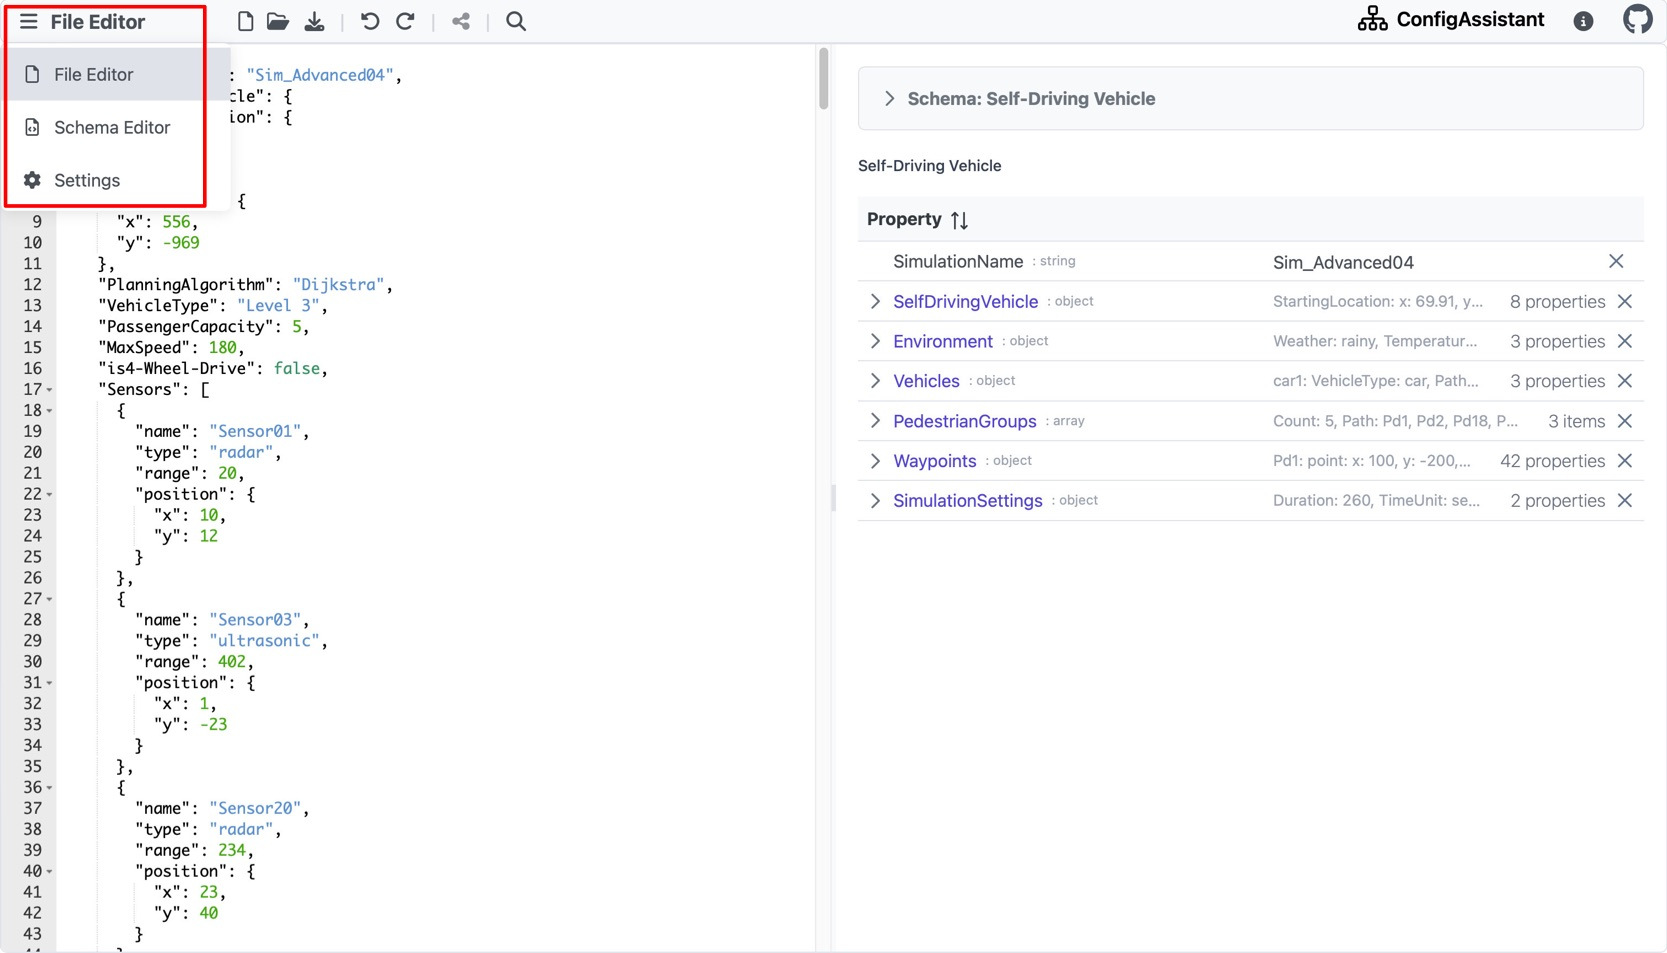
\includegraphics[width=3.5in]{figures/Views}
\end{minipage}

While these views share a similar appearance, right side GUI Panel and left side Code Panel,
\begin{figure}[h]
    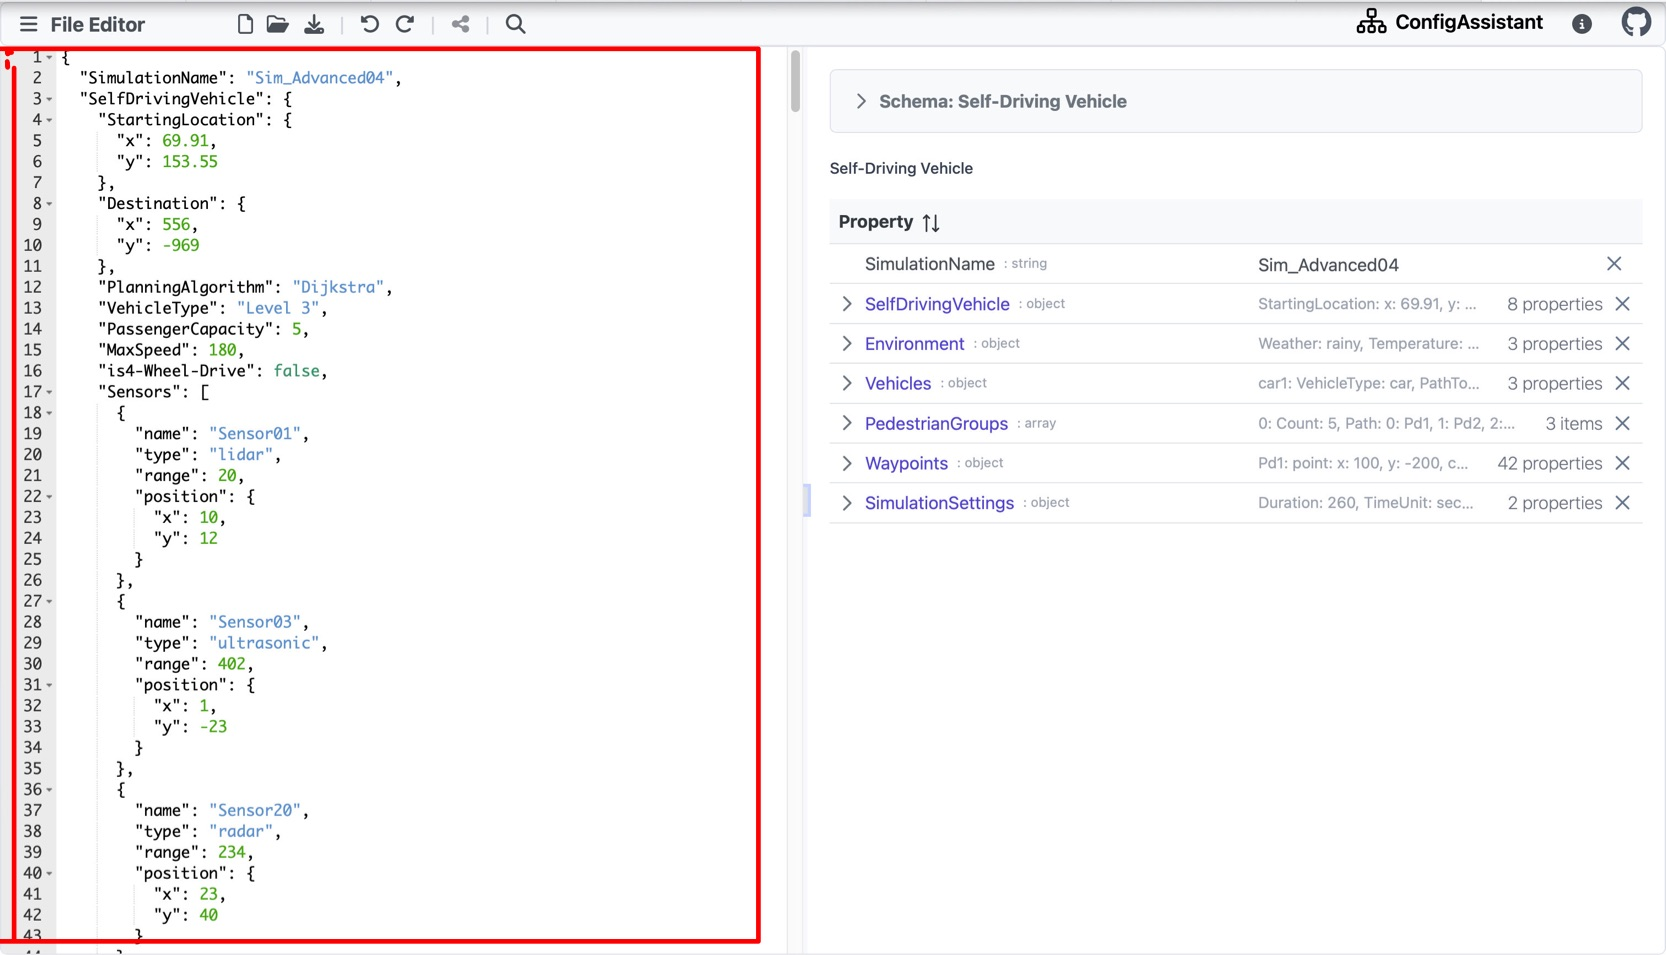
\includegraphics[width=3.5 in]{figures/Code Panel}
    \caption{Code Panel}
\end{figure}
\begin{figure}[h]
    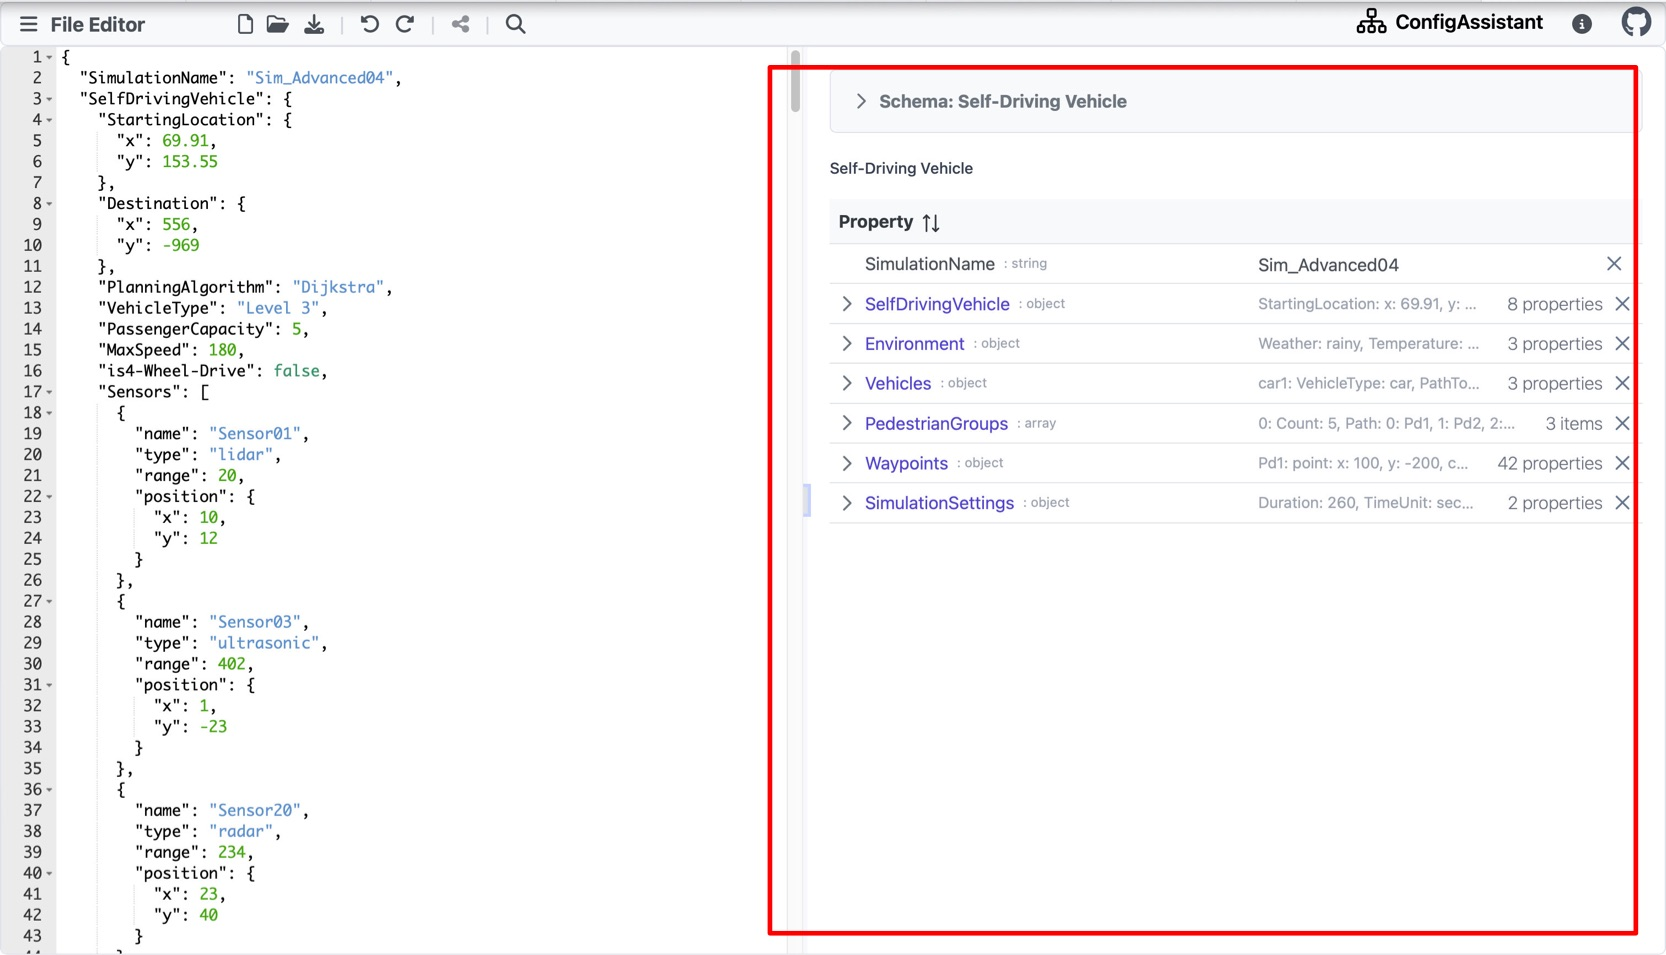
\includegraphics[width=3.5 in]{figures/GUI Panel.jpg}
    \caption{GUI Panel}
\end{figure}
each serves a different purpose, which we discuss in the following.

\subsubsection{File Editor}
The File Editor view is primarily designed for creating and editing configuration files.It features a user-friendly top menu bar that provides various essential functionalities:
\begin{figure}[h]
    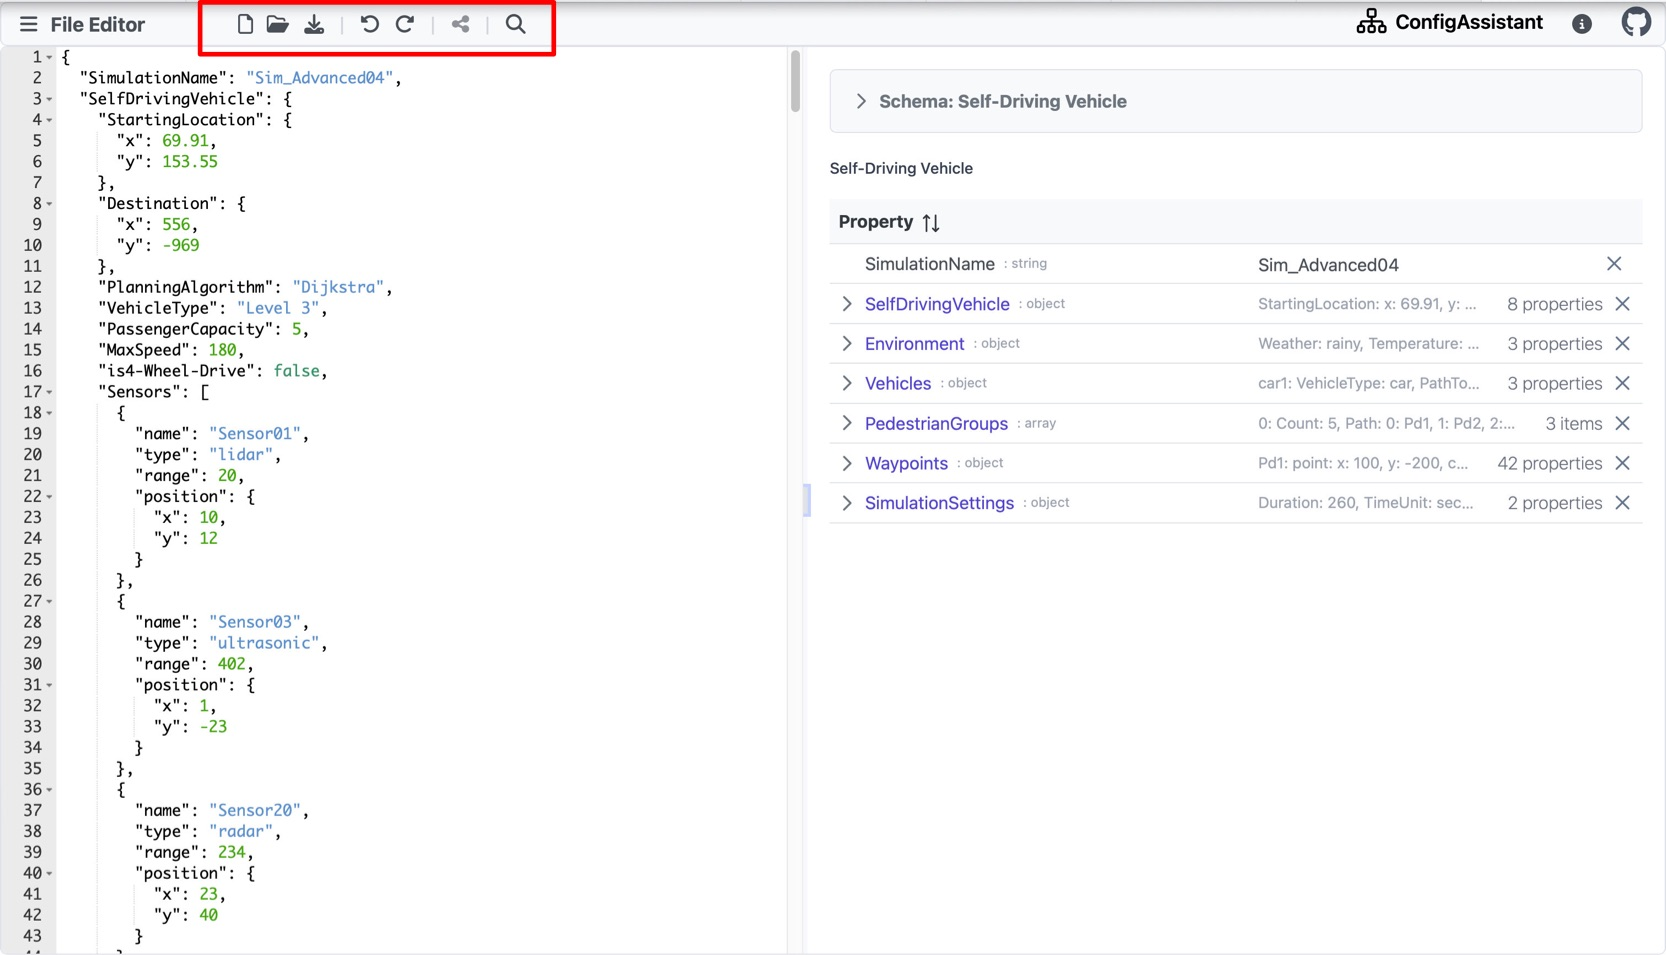
\includegraphics[width=3.5 in]{figures/FileeditorTopmenubar}
    \caption{FileEditor Topmenubar}
\end{figure}

\begin{itemize}
    \item \textbf{New File:} Create a new configuration file. This option also includes two subitems:
    \begin{itemize}
        \item \textbf{Generate Data:} Generate random configuration data based on the selected schema from the Schema Editor.
        \item \textbf{New Empty File:} Start with a blank configuration file, discarding any current changes.
    \end{itemize}
\end{itemize}

\begin{itemize}
    \item \textbf{Open File:} Open an existing configuration file from local storage.
\end{itemize}
\begin{itemize}
    \item \textbf{Undo/Redo:} Easily undo or redo actions to manage changes effectively.
\end{itemize}
\begin{itemize}
    \item \textbf{Download Config:} Download the current configuration with an appropriate file name.
\end{itemize}
\begin{itemize}
    \item \textbf{Search:} Utilize the search option to quickly find and navigate to specific keywords or sections within user's configuration files.
\end{itemize}

\subsubsection{Schema Editor}

The Schema Editor view allows users to define and manage schema templates for configuration files. 
This view is essential for maintaining consistency and structure within your configurations. 
% Details of the Schema Editor and its functionalities can be inserted here.

\begin{figure}[h]
    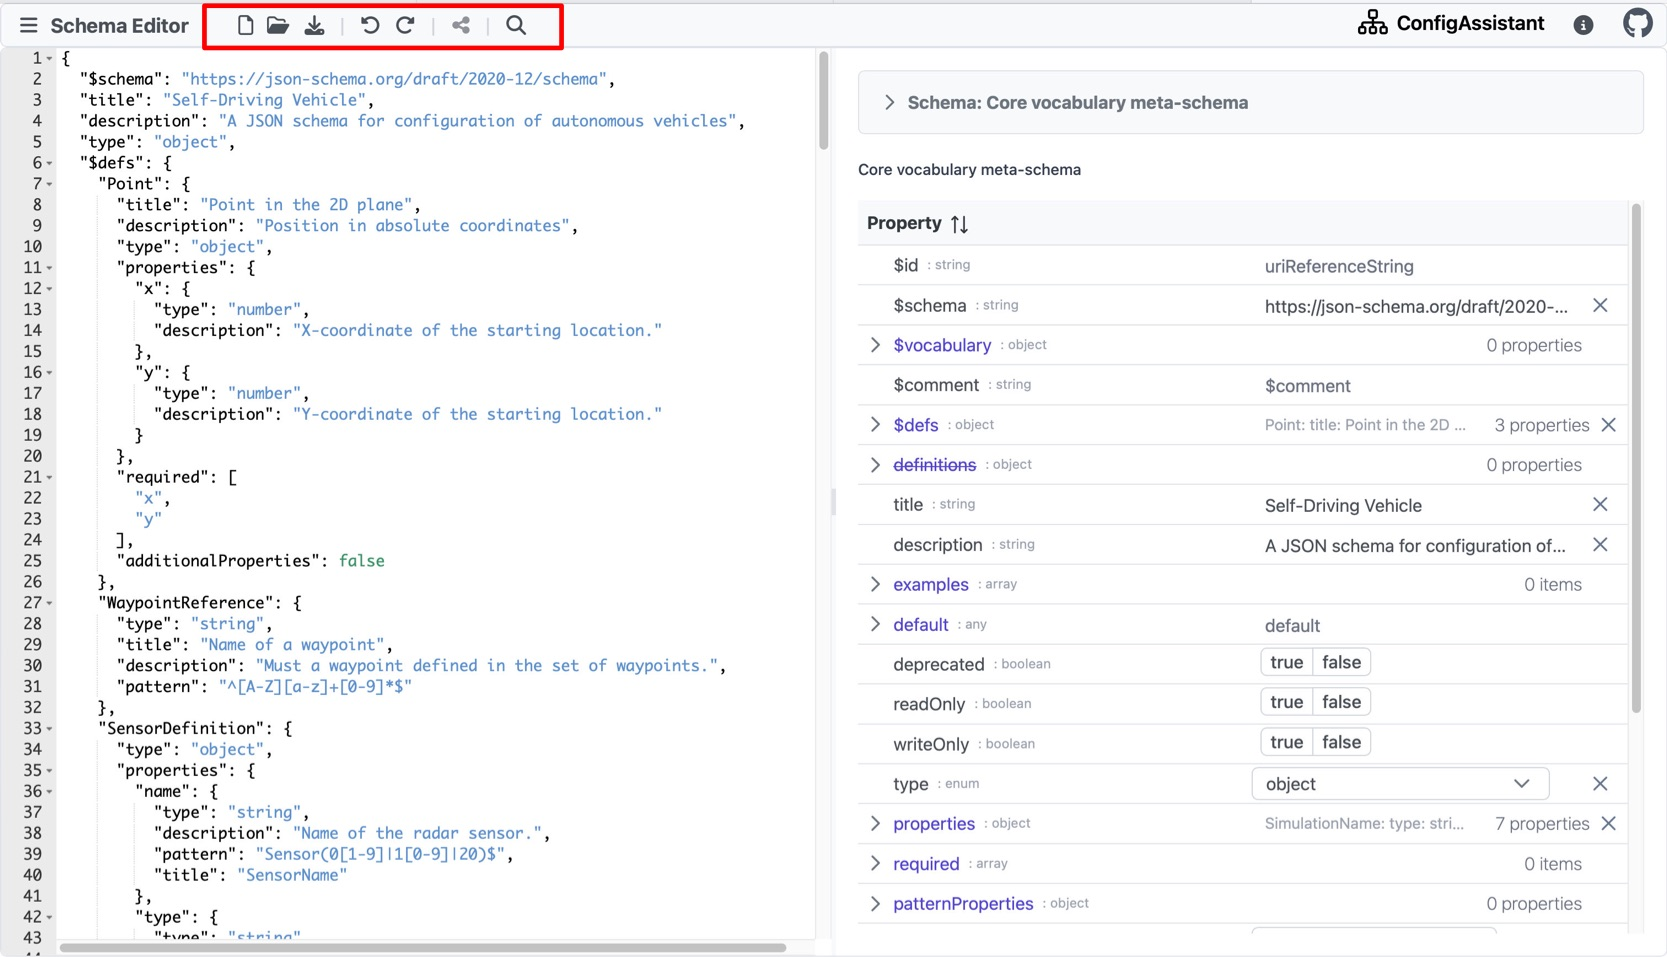
\includegraphics[width=3.5 in]{figures/Schemaeditor Topmenubar}
    \caption{SchemaEditor Topmenubar}
\end{figure}

\begin{itemize}
    \item \textbf{New Empty Schema:} Clear the current schema for starting fresh.
\end{itemize}

\begin{itemize}
    \item \textbf{Open Schema:} Open an existing schema, offering four suboptions:
    \begin{itemize}
        \item \textbf{JSON Schema Store:} Choose a schema from the JSON Schema Store, which provides a list of available schemas.

        \item \textbf{From Our Examples:} Access four example schemas provided within the tool.

        \item \textbf{From File:} Select a schema from local file system.

        \item \textbf{From URL:} Provide the URL of a specific schema, and the tool will retrieve and open it.

    \end{itemize}
\end{itemize}

\begin{itemize}
    \item \textbf{Download Schema:} Download the current schema for later use or reference.
\end{itemize}
\begin{itemize}
    \item \textbf{Undo/Redo:} Easily undo or redo actions to manage schema changes effectively.

\end{itemize}
\begin{itemize}
    \item \textbf{Search:} Utilize the search option to quickly find and navigate within user's schema definitions, enhancing schema management.
\end{itemize}

\subsubsection{Settings}

The Settings view provides customization options for tailoring the tool to your specific needs. 
It allows user to configure various preferences and settings to enhance user's workflow.
% Details of the Settings view and its functionalities can be inserted here.
\begin{figure}[h]
    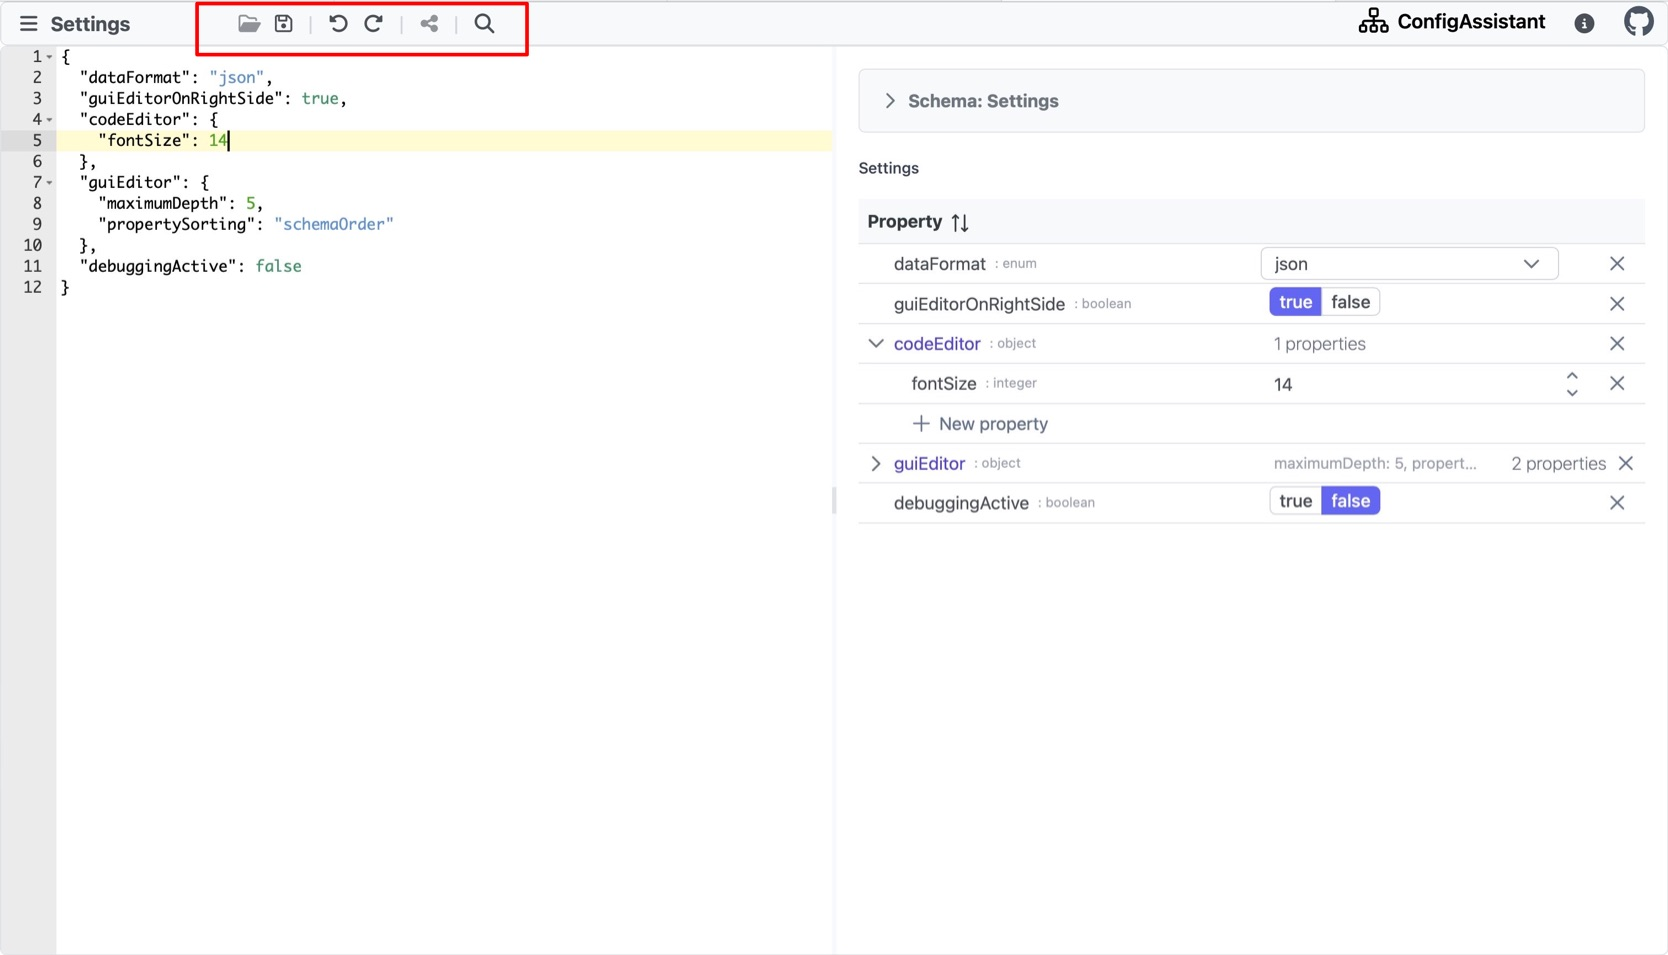
\includegraphics[width=3.5 in]{figures/Settings Topmenubar}
    \caption{Settings Topmenubar}
\end{figure}
\begin{itemize}
    \item \textbf{Save:} Save the current Settings that user configured.
    \item \textbf{Undo/Redo:} Quickly undo or redo actions related to configuration settings adjustments.
    \item \textbf{Search:} Utilize the search option to find specific configuration settings or preferences efficiently.
\end{itemize}

The Settings view allows users to configure various settings:
\begin{figure}[h]
    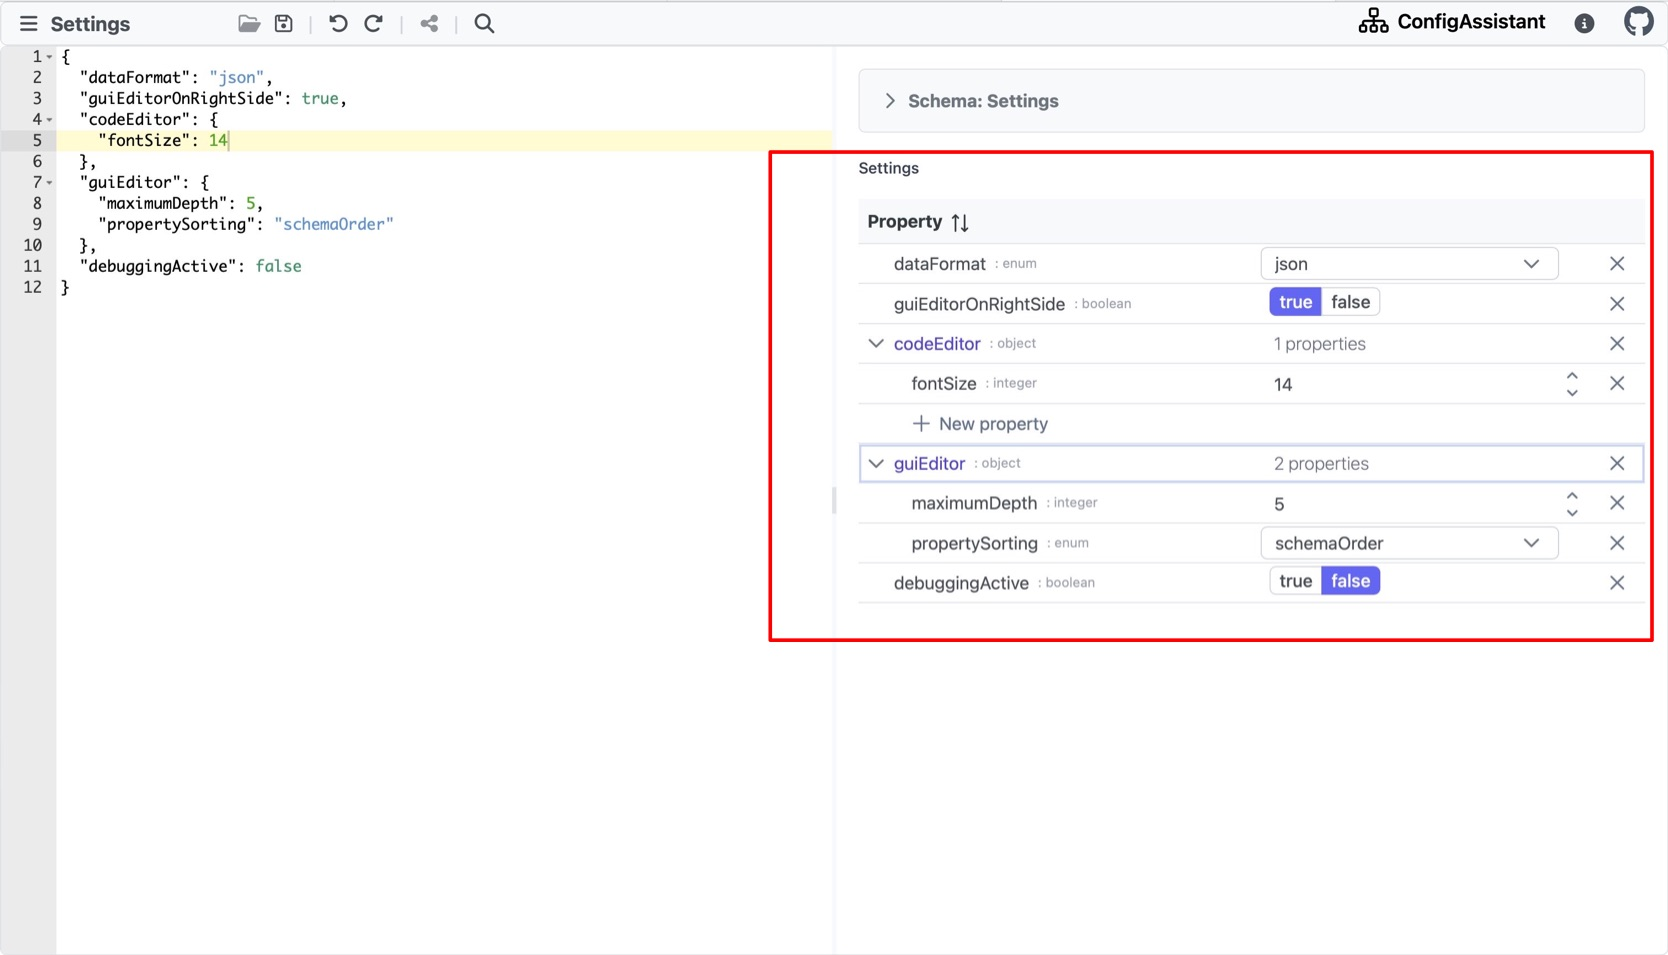
\includegraphics[width=3.5 in]{figures/GUI Editor Pannel Settings}
    \caption{Settings's GUI Pannel}
\end{figure}
\begin{itemize}
    \item \textbf{Data Format:} Users can select between JSON and YAML data format.
    The choice made here will influence all three views.
    \item \textbf{GuiEditorOnRightSide:} By default, the GUI panel is located on the right side, but users have the flexibility to change it to the left side using the \textbf{guiEditorOnRightSide} option.
    \item \textbf{Code Editor Font Size:} Customize the font size in the code editor panel to suit user's preferences.
    \item \textbf{GUI Editor Configuration:} Users can configure the \textbf{maximum depth} and \textbf{property sorting} in the GUI editor, including options like \textbf{Schema Order}, \textbf{Priority Order}, and \textbf{Data Order}.
    \begin{itemize}
        \item \textbf{Schema Order:} Define the order in which schema elements are presented.
        \item \textbf{Priority Order:} Customize the order of elements based on their priority.
        \item \textbf{Data Order:} Specify the order in which data elements are displayed.
    \end{itemize}
    \item \textbf{Debugging Panel:} For debugging purposes, users can enable or disable the debugging panel as needed.
\end{itemize}

\subsection{Workflow}\label{subsec:workflow}
In this section, we outline the workflow of our tool.

\begin{enumerate}
    \item Users can access our tool by visiting the following link: \href{https://paulbredl.github.io/config-assistant/}{ConfigAssistant}.
    \item Upon initial access, a default page is displayed, and users must select their desired Schema. 
    We have implemented four options for this selection:
    \begin{enumerate}
        \item From File
        \item From JSON Store
        \item From URL
        \item From Our Example
    \end{enumerate}
    Users can make their Schema selection either via a dialog box on the default page or in the schema Editor.
    \item After selecting a schema, the user will find that a GUI is automatically generated on the right-hand side of the File Editor, tailored to the selected schema.
    \item Through the GUI panel, users are assisted in creating or modifying configuration files effortlessly, ensuring a seamless configuration file generation process.
    \item If a user wishes to modify the selected schema, such as adding new properties, they can do so through the schema editor. Changes can be made using either the GUI panel or the code panel, and these modifications will automatically reflect in the file editor.
\end{enumerate}

Furthermore, users have the option to explore our Settings view, where they can change the Schema Language (e.g., JSON or YAML) and configure other settings to suit their preferences.

\begin{figure}[!htb]
    \begin{minipage}[t]{0.5\textwidth}
        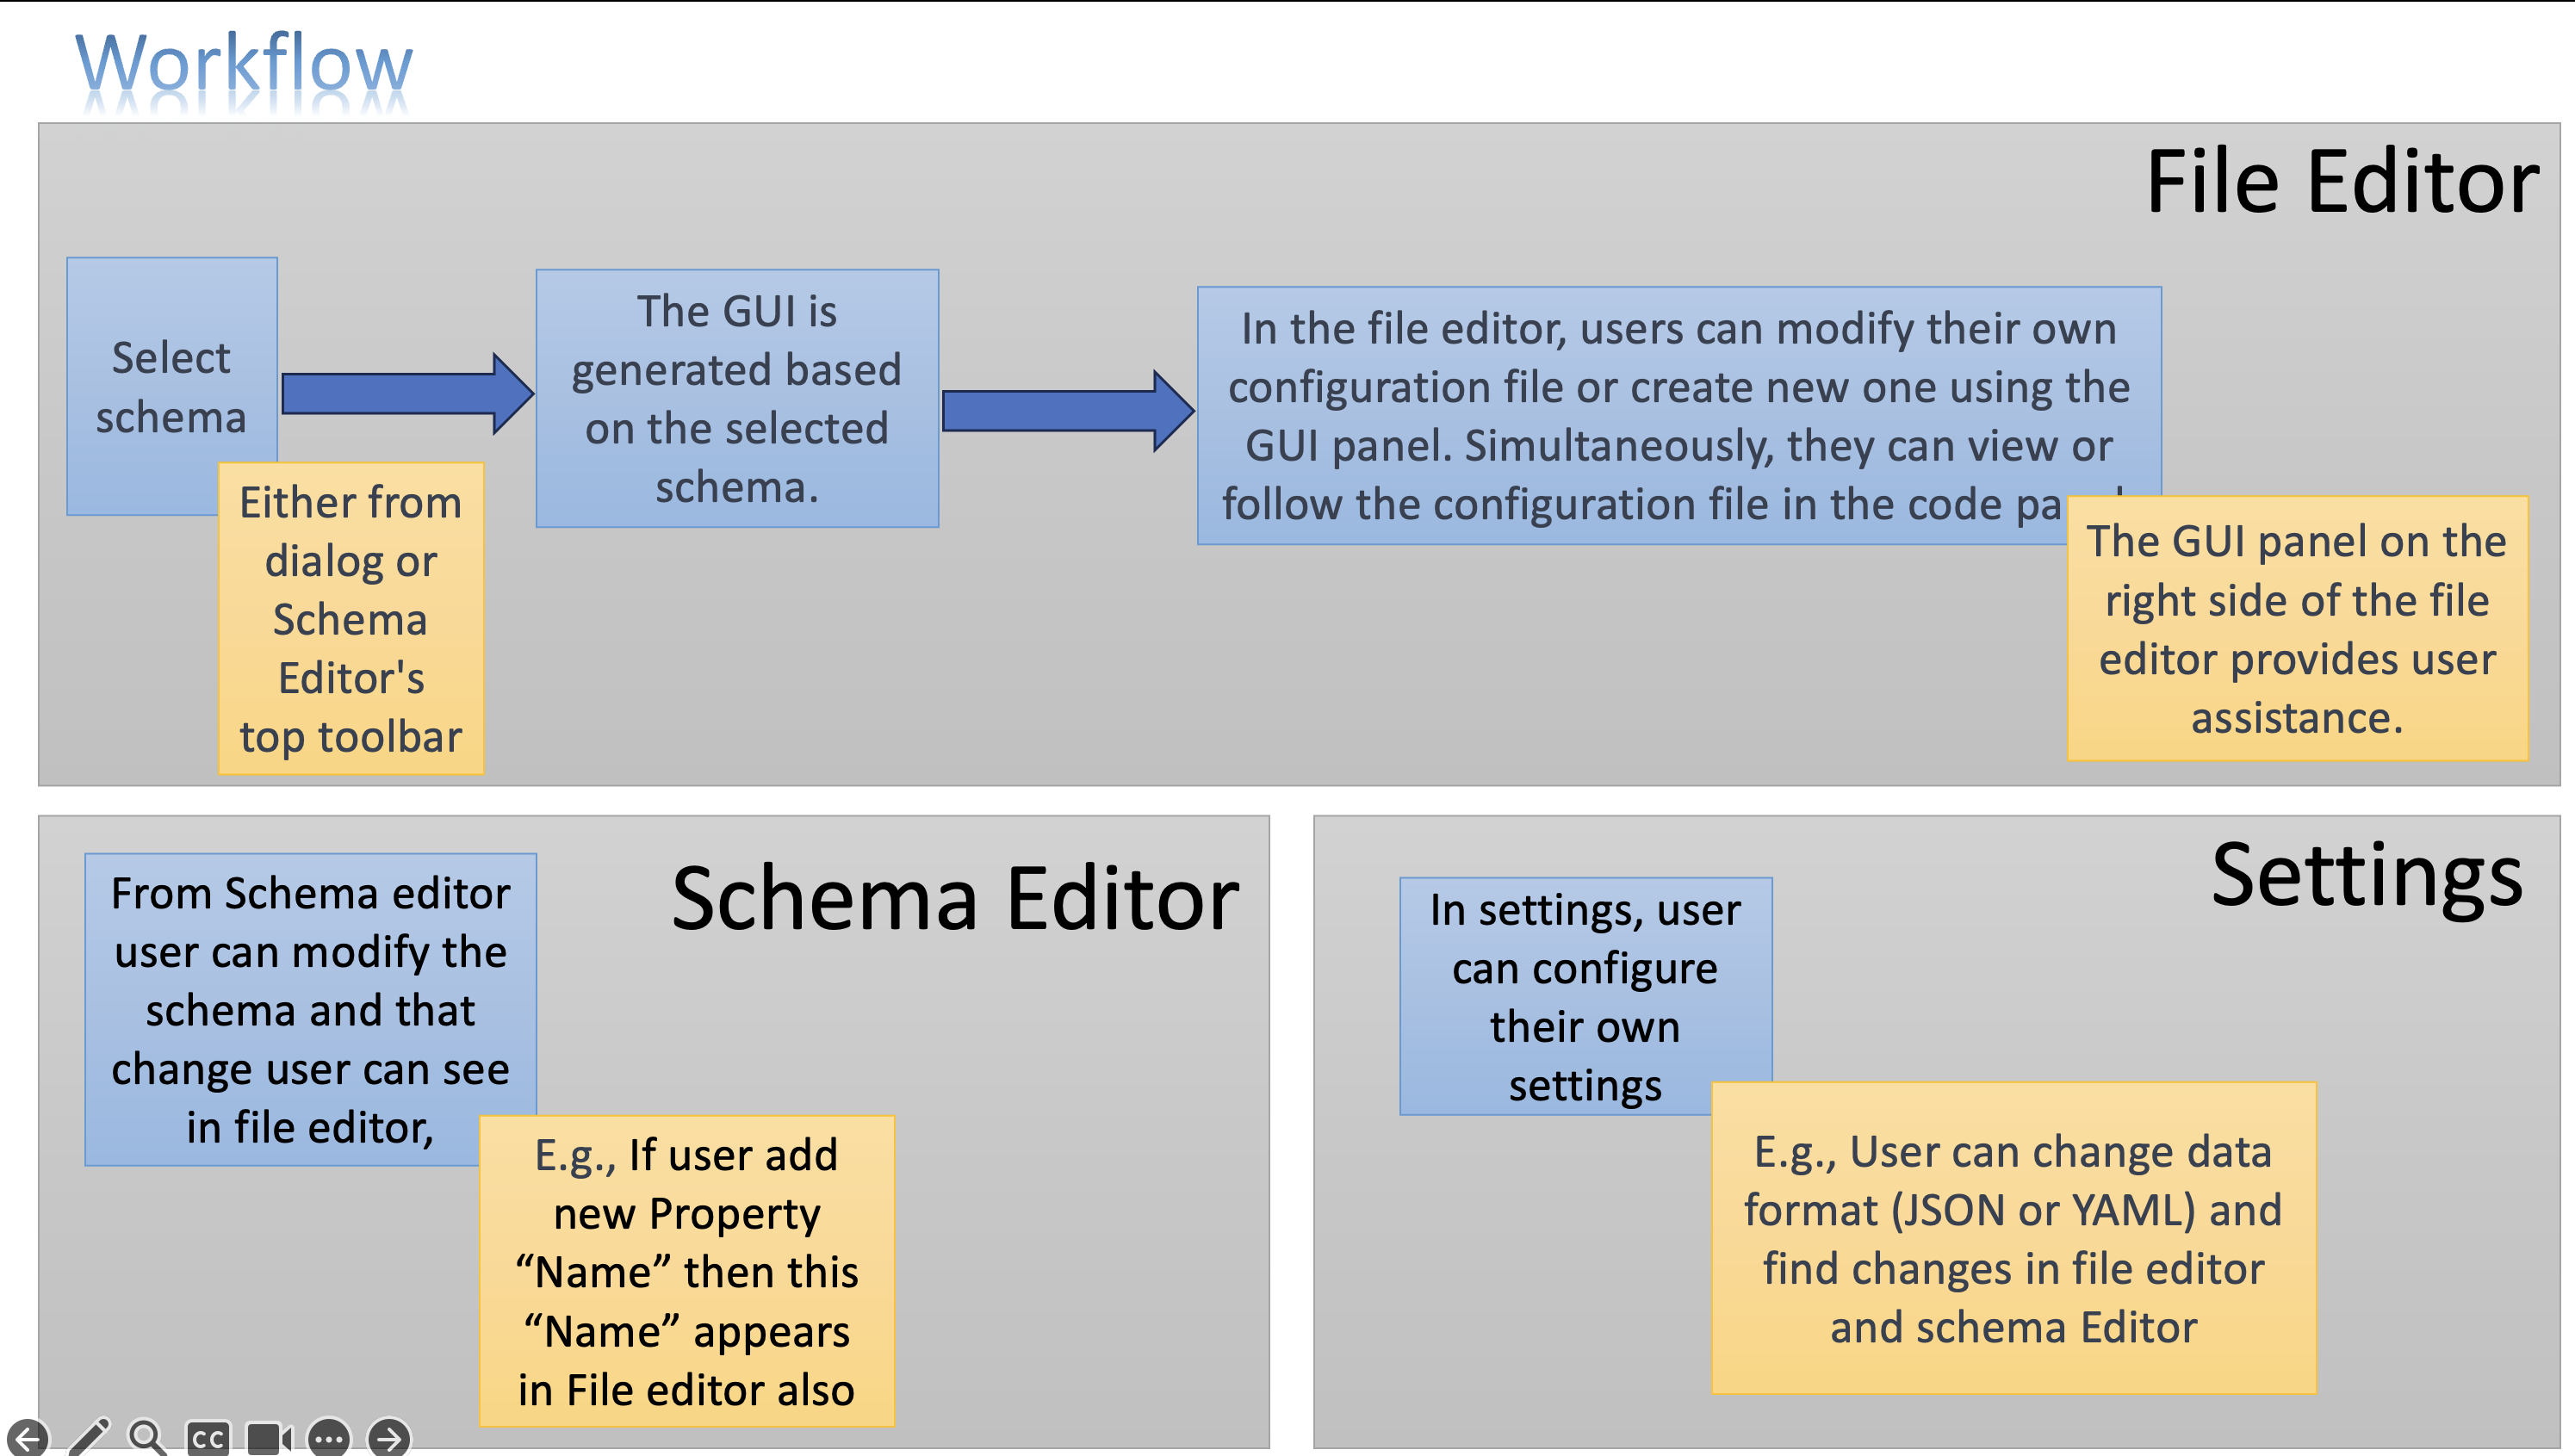
\includegraphics[width=3.5in]{figures/workflow}
        \caption{Workflow}
    \end{minipage}\label{fig:workflow}
\end{figure}

\subsection{Code Editor}\label{subsec:code-editor}

% todo decribe the code editor component and how it works

\subsection{GUI Editor}\label{subsec:gui-editor}

The GUI editor is a component that allows the user to edit the configuration data in a GUI, which is generated based on the schema of the configuration data.
It is structured in a table-like way, where each row represents a key-value pair of the configuration data.
Arrays elements are represented similarly, where the index of the array element is the key and the value is the array element itself.
Figure~\ref{fig:gui-editor} shows the GUI editor component with an example schema and configuration data.

\begin{figure}[!t]
    \centering
    \includegraphics[width=\columnwidth]{figures/gui-editor} % todo replace with screenshot
    \caption{GUI Editor Component}
    \label{fig:gui-editor}
\end{figure}

To allow this representation of the schema, we do some preprocessing of the \textbf{schema}, which is described in section~\ref{subsec:schema-preprocessing}.

\subsubsection{Features}\label{subsubsec:gui-editor-features}

To assist the user in editing the configuration data, the GUI editor offers a set of features, which are described in the following.

\paragraph{Traversal of the Data Tree}
By default, only the first level of the data tree is shown.
The user can expand the data tree by clicking on the arrow next to the key of an object or array.
This will show the sub-properties of the object or the elements of the array.
We limit the depth of the data tree to a configurable value, to prevent the GUI editor becoming too overwhelming.
However, the user can also click on the property name or array index to \textit{zoom in} to that element.
This will show the sub-properties of that element at the top level, as if that property was the root of the data tree.
The breadcrumb at the top allows the user to see which path the GUI editor currently shows and to navigate back to upper levels of the tree.

% todo add figure to illustrate

\paragraph{Type specific components}

% todo write

\paragraph{Remove Data}
The user can delete properties or array elements from the data by clicking on the $\times$ button next to the edit field.
This button is only shown if the property is not required.

\paragraph{Schema Information Tooltip}
When the user hovers over the property key or array index, an overlay is displayed which contains all information from the schema about that property.
We manually implemented a generation of a textual description for each of the JSON schema keywords.
This feature helps the user to understand the constraints and the meaning of a property.

\paragraph{Highlighting Schema Validation Errors}
When the configuration data does not comply to the schema, the corresponding elements are underlined in red.
This way, the user knows where any errors are.
Additionally, when hovering over the property name, more details about the error are shown.
% todo add screenshot

\subsection{Schema preprocessing}\label{subsec:schema-preprocessing}

To represent the schema in the GUI editor, we preprocess the schema.
We differentiate between three ways of preprocessing:
A one-time preprocessing step when loading the schema, an internal preprocessing that happens at every layer of the schema tree,
and calculating an effective schema that happens everytime the configuration data changes.

\subsubsection{One-time Preprocessing Step}
When the schema is loaded, we perform a one-time preprocessing step that currently only involves migrating the schema to the newest version,
as described in section~\ref{subsec:json-schema-versions}.
The user will be informed about this step and also prompted with a dialog, when the schema file does not define which JSON schema version it uses.
After the migration, the resulting schema is loaded into the tool in the \textit{Schema Editor} page.

% todo maybe describe how bundling might make sense here

\subsubsection{Internal preprocessing}
This preprocessing steps are mainly used to generate the GUI editor and thus are internal steps that will not be visible for the user.
They happen at every layer of the schema tree lazily, only when required.
This lazy preprocessing is required as schemas can have circular references, which would lead to infinite loops.
In the following, we describe the preprocessing steps in details.

\paragraph{Resolving references}
JSON schema uses the \texttt{\$ref} keyword to reference other schemas.
This can either be references to schemas in the same file (using the \texttt{\$defs} keyword), references to other local files,
or references to schemas at a URL in the web.
We currently only support references to schemas in the same file.
These are lazily resolved as the first preprocessing step.
Listing~\ref{listing:preprocessing-example} shows an example schema, Listing~\ref{listing:reference-resolving} shows the equivalent example after
this first preprocessing step.

\begin{listing}[!h]
    \begin{minted}[frame=single,
        framesep=3mm,
        linenos=true,
        xleftmargin=15pt,
        tabsize=4]{js}
{
  "title": "NonEmptyString",
  "$ref": "#/$defs/nonEmptyString",
  "$defs": {
    "nonEmptyString": {
      "type": "string",
      "minLength": 1
     }
  }
}
    \end{minted}
    \caption{Simple JSON schema before reference resolving}
    \label{listing:preprocessing-example}
\end{listing}

\begin{listing}[!h]
    \begin{minted}[frame=single,
        framesep=3mm,
        linenos=true,
        xleftmargin=15pt,
        tabsize=4]{js}
{
  "allOf": [
   {
     "title": "NonEmptyString"
   },
   {
     "type": "string",
     "minLength": 1
   }
  ],
  "$defs": {
    "nonEmptyString": {
      "type": "string",
      "minLength": 1
     }
  }
}
    \end{minted}
    \caption{Simple JSON schema after reference resolving}
    \label{listing:reference-resolving}
\end{listing}

\paragraph{Resolving allOfs}

The \texttt{allOf} keyword in JSON schema specifies that all of the schemas in the given array must be valid.
To simplify any other operation on the schema, we aim to merge the schemas in the allOf array to one equivalent schema.
As the first step, we do a recursive step by preprocessing all the schemas of the allOf array.
Then, we use the \textit{mergeAllOfs} library % todo citation
for this task.
Listing~\ref{listing:resolved-allOf} shows the previous example schema after this step.
It is important to note that this library only supports a few keywords of JSON schema, most notably the
\texttt{properties} and \texttt{items} keyword.
Hence, the support for allOf and any other keywords for which we use this in the preprocessing is limited.

\begin{listing}[!h]
    \begin{minted}[frame=single,
        framesep=3mm,
        linenos=true,
        xleftmargin=15pt,
        tabsize=4]{js}
{
  "title": "NonEmptyString"
  "type": "string",
  "minLength": 1,
  "$defs": {
    "nonEmptyString": {
      "type": "string",
      "minLength": 1
     }
  }
}
    \end{minted}
    \caption{Simple JSON schema after allOf resolving}
    \label{listing:resolved-allOf}
\end{listing}

\paragraph{anyOf and oneOf} % todo

\paragraph{Title inducing}

The \texttt{title} keyword is used to give a schema a short description.
This is not necessarily the same as the property name of properties of an object.
As we use the title in various cases to display for the user, we inject the property name in cases where no explicit title is given.

\begin{listing}[!h]
    \begin{minted}[frame=single,
        framesep=3mm,
        linenos=true,
        xleftmargin=15pt,
        tabsize=4]{js}
{
  "type": "object",
  "properties": {
    "name": {
        "type": "string"
    }
  }
}
    \end{minted}
    \caption{Simple JSON schema with one property without a title}
    \label{listing:no-title}
\end{listing}

\begin{listing}[!h]
    \begin{minted}[frame=single,
        framesep=3mm,
        linenos=true,
        xleftmargin=15pt,
        tabsize=4]{js}
{
  "type": "object",
  "properties": {
    "name": {
        "title": "name",
        "type": "string"
    }
  }
}
    \end{minted}
    \caption{The property names was used for the title field}
    \label{listing:with-title}
\end{listing}

\paragraph{Processing enum and const}
The enum keyword is used to restrict the values of a field to a fixed set of valid values.
The const keyword, similarly, restricts the property value to a single allowed value.
Thus, setting the const value is equivalent to settings the enum value with an array that contains this single value.

We convert any usage of const to enums with a single element, which allows us to ignore the const keyword in other operations.

\subsubsection{Calculating an effective schema}

This third preprocessing step is calculated the most often, namely every time the data changes.
However, for most schemas this preprocessing step is trivial.
The JSON schema keywords \texttt{if}, \texttt{then}, and \texttt{else} provide a way to include conditions in the JSON schema.
If the schema in the \texttt{if} field is valid, then also the schema in the \texttt{then} field must be valid, otherwise the
schema in the \texttt{else} field must be valid.

This makes the schema data dependent.
To show the correct properties, we evaluate the data and dependent on validity or not, we either use the \texttt{then} or the \texttt{else} schema.

We similarly handle the \texttt{dependentRequired} and the \texttt{dependentSchemas} keywords.
For schemas without any of those keywords, this step is trivial as the schema is not modified in any way.

%todo examples

\subsubsection*{\bf A plain unnumbered list}
\begin{list}{}{}
    \item{bare\_jrnl.tex}
    \item{bare\_conf.tex}
    \item{bare\_jrnl\_compsoc.tex}
    \item{bare\_conf\_compsoc.tex}
    \item{bare\_jrnl\_comsoc.tex}
\end{list}

\subsection{Figures}
Fig. 1 is an example of a floating figure using the graphicx package.
Note that $\backslash${\tt{label}} must occur AFTER (or within) $\backslash${\tt{caption}}.
For figures, $\backslash${\tt{caption}} should occur after the $\backslash${\tt{includegraphics}}.

%\begin{figure}[!t]
%\centering
%\includegraphics[width=2.5in]{fig1}
%\caption{Simulation results for the network.}
%\label{fig_1}
%\end{figure}

Fig. 2(a) and 2(b) is an example of a double column floating figure using two subfigures.
(The subfig.sty package must be loaded for this to work.)
The subfigure $\backslash${\tt{label}} commands are set within each subfloat command,
and the $\backslash${\tt{label}} for the overall figure must come after $\backslash${\tt{caption}}.
$\backslash${\tt{hfil}} is used as a separator to get equal spacing.
The combined width of all the parts of the figure should do not exceed the text width or a line break will occur.
%
%\begin{figure*}[!t]
%\centering
%\subfloat[]{\includegraphics[width=2.5in]{fig1}%
%\label{fig_first_case}}
%\hfil
%\subfloat[]{\includegraphics[width=2.5in]{fig1}%
%\label{fig_second_case}}
%\caption{Dae. Ad quatur autat ut porepel itemoles dolor autem fuga. Bus quia con nessunti as remo di quatus non perum que nimus. (a) Case I. (b) Case II.}
%\label{fig_sim}
%\end{figure*}

Note that often IEEE papers with multi-part figures do not place the labels within the image itself (using the optional argument to $\backslash${\tt{subfloat}}[]), but instead will
reference/describe all of them (a), (b), etc., within the main caption.
Be aware that for subfig.sty to generate the (a), (b), etc., subfigure
labels, the optional argument to $\backslash${\tt{subfloat}} must be present. If a
subcaption is not desired, leave its contents blank,
e.g.,$\backslash${\tt{subfloat}}[].